\chapter{REVISIÓN DE LITERATURA}
\label{cap:3}

\section{Definición de términos clave}
\begin{definition}[Precipitación]
 Fenómeno meteorológico que ocurre en sistemas a pequeña escala, caracterizado por la formación de nubes del tipo cúmulus bajo condiciones específicas: presencia de núcleos de condensación, temperaturas cercanas al punto de rocío y un abasto continuo de vapor de agua. A medida que las gotas aumentan de tamaño mediante colisiones, pueden generarse diversas manifestaciones, como lluvia, granizo, nieve, trombas, tornados, rayos y truenos  (\cite{ahrens2020}).
\end{definition}

\begin{definition}[Lluvia]
    Es la caída de agua procedente de las nubes en estado líquido, sólido y semisólido (\cite{breña2013}).
\end{definition}


El monitoreo es fundamental para la toma de decisiones informadas en la gestión ambiental y otros campos.
\begin{definition}[Monitoreo]
  Es un proceso sistemático y continuo que permite observar, registrar y analizar parámetros específicos para evaluar el estado o cambios en un sistema o fenómeno determinado.(\cite{ciga_monitoreo})
\end{definition}


\begin{definition}[Ciencia Ciudadana]
Es una metodología científica que involucra activamente a la ciudadanía en la generación de conocimiento, permitiendo que personas sin formación científica formal participen en la recolección, análisis e interpretación de datos, contribuyendo así a proyectos de investigación y al fomento de la cultura científica.(\cite{csic_ciencia_ciudadana})
\end{definition}


\begin{definition}[Flutter]
Flutter es un framework de código abierto desarrollado por Google que permite crear aplicaciones nativas de alto rendimiento para múltiples plataformas (iOS, Android, web, escritorio) a partir de una única base de código, utilizando el lenguaje de programación Dart.(\cite{flutter_multiplataforma})
\end{definition}

\begin{definition}[Dart]

Dart es un lenguaje de programación desarrollado por Google, diseñado para crear aplicaciones frontend rápidas y optimizadas, especialmente utilizado en conjunto con Flutter. (\cite{dart})
\end{definition}

\begin{definition}[Widget]

Los widgets son los componentes básicos de la interfaz de usuario de una aplicación de Flutter, y cada widget es una declaración inmutable de una parte de la interfaz. Los widgets se utilizan para describir todos los aspectos de una interfaz de usuario, incluyendo aspectos físicos como texto y botones para diseñar efectos como el relleno y la alineación. (\cite{flutter_multiplataforma})
\end{definition}



\begin{definition}[Firebase]

Firebase es una plataforma de desarrollo de aplicaciones creada por Google que proporciona servicios como bases de datos en tiempo real, autenticación de usuarios, hosting de archivos y funciones de backend sin servidor, facilitando el desarrollo y escalamiento de aplicaciones móviles y web. (\cite{firebase})
\end{definition}


\begin{definition}[Backend]
El backend se refiere a la parte del desarrollo de software que gestiona la lógica de negocio, bases de datos, servidores y APIs, funcionando como la estructura interna que sostiene y conecta los servicios de una aplicación.(\cite{backend})
\end{definition}



\begin{definition}[Frontend]
  El frontend es la capa de una aplicación que interactúa directamente con el usuario, encargándose del diseño, la estructura y la experiencia visual mediante tecnologías como HTML, CSS y JavaScript o frameworks como Flutter para móviles.(\cite{frontend})
\end{definition}


\begin{definition}[GitHub]
  \textit{GitHub} es una plataforma de desarrollo colaborativo que permite a los desarrolladores alojar proyectos, gestionar versiones mediante Git, colaborar en equipos, revisar código y automatizar flujos de trabajo. Su integración con Git permite el control detallado de versiones, ramas y contribuciones en proyectos de software. Además, ofrece funcionalidades como GitHub Actions, Issues, Pull Requests y GitHub Pages, lo que la convierte en un entorno completo para el desarrollo y la gestión de proyectos de código abierto y privado  (\cite{githubdocs}).
\end{definition}


\begin{definition}[Google Play Console]
  Google Play Console es la plataforma de gestión que permite a los desarrolladores publicar, actualizar, monitorear el rendimiento y administrar la distribución de sus aplicaciones Android en la tienda Google Play.(\cite{googleplayconsole})


\end{definition}

\begin{definition}[Firebase Realtime Database]
Es un servicio de base de datos en la nube que almacena y sincroniza datos entre usuarios en tiempo real, ideal para aplicaciones que requieren actualizaciones inmediatas. (\cite{firebaserealtime})
\end{definition}

\begin{definition}[User Interface (UI)]
  La \textit{interfaz de usuario} (UI, por sus siglas en inglés) es la capa visual e interactiva de una aplicación o sistema digital, diseñada para facilitar la interacción del usuario con las funcionalidades internas del software. Comprende todos los elementos gráficos visibles como botones, formularios, menús, iconos, gráficos y controles que permiten a los usuarios ejecutar tareas específicas. Una UI bien diseñada se enfoca en la usabilidad, accesibilidad, estética y eficiencia, siendo un componente esencial en la experiencia del usuario  (\cite{shneiderman}).
\end{definition}



\begin{definition}[Material Design]
Material Design es un sistema de diseño desarrollado y respaldado por diseñadores y desarrolladores de Google. Material.io incluye una guía detallada de UX e implementaciones de componentes de UI para Android, Flutter y la web.

La última versión, Material 3, permite experiencias personales, adaptables y expresivas, desde colores dinámicos y accesibilidad mejorada hasta bases para diseños de pantalla grande y tokens de diseño. M3 Expressive va un paso más allá al añadir componentes más flexibles, estilos vibrantes y movimiento totalmente integrado. (\cite{materialdesign2023})
\end{definition}

\begin{definition}[Pluviómetro manual]

El pluviómetro manual es un instrumento utilizado para medir la cantidad de precipitación líquida caída en un lugar específico durante un período determinado. Consiste en un recipiente cilíndrico que recoge el agua de lluvia, la cual se mide posteriormente con una probeta graduada. Este instrumento debe cumplir con las especificaciones establecidas en las normas mexicanas para garantizar la precisión y confiabilidad de los datos obtenidos.(\cite{semarnat_pluviometro})
\end{definition}

Las especificaciones para construir un pluviómetro (Figura \ref{t1}), son las siguientes:
\begin{itemize}
    \item El depósito debe tener una entrada estrecha, suficientemente protegida de la radiación, para reducir al mínimo las pérdidas de agua por evaporación
    \item Este instrumento debe colocarse en lugares abiertos y su área de captación debe permanecer horizontal y a 100 cm del suelo. (\cite{se2013})
\end{itemize}

\begin{figure}[h!]
\centering
  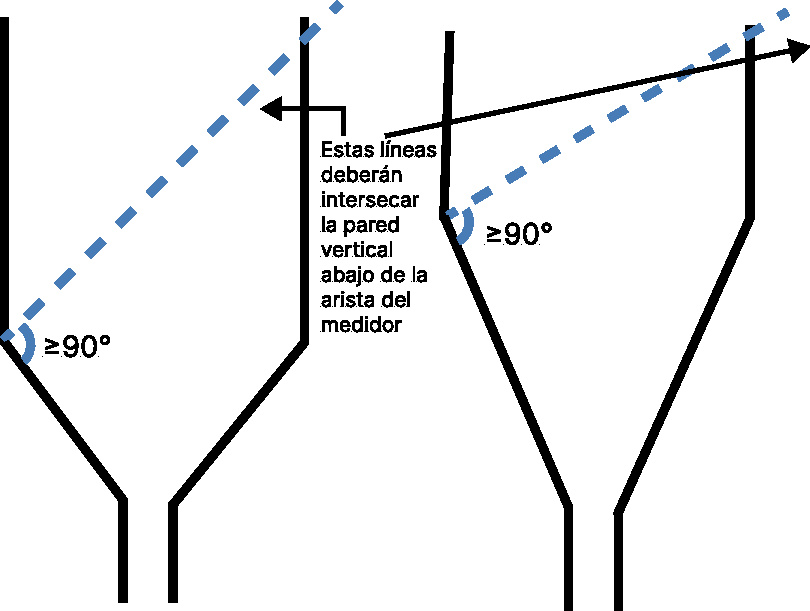
\includegraphics[width=0.5\textwidth]{t1.pdf}
  \caption{Colectaros adecuados para los pluviómetros según la norma NMX-AA-166/1-SCFI-2013 (\cite{se2013})}
  \label{t1}
\end{figure}


\newpage


\section{Acceso a datos meteorológicos de zonas de montaña en México}

\subsection{Antecedentes en el Monte Tláloc}

En mayo de 2012, la Universidad Autónoma del Estado de México (UAEM), en coordinación con el INAH y autoridades locales, impulsó la creación de una Estación de Investigación Ambiental y Monitoreo Meteorológico (EIAMM) en el Monte Tláloc, a más de 4,200 ms.n.m. El objetivo era analizar tendencias climáticas regionales y generar alertas tempranas ante posibles eventos extremos, especialmente lluvias intensas que pudieran impactar el Valle de México  (\cite{davila2012}). Sin embargo, no se encontraron publicaciones científicas posteriores que reportaran el funcionamiento de estaciones meteorológicas permanentes en ese sitio. Por tanto, este proyecto constituye un antecedente significativo, aunque no se llegó a consolidar con datos operativos documentados.

No se encontraron artículos científicos que reporten monitoreo climatológico temporal o permanente en Monte Tláloc mediante estaciones meteorológicas oficiales (CONAGUA, universidades, etc.).


\subsection{Panorama a nivel nacional}

Aunque el monitoreo meteorológico en zonas montañosas de México ha sido limitado históricamente, en las últimas décadas se han realizado diversos esfuerzos por parte de instituciones académicas, gubernamentales y ciudadanas para instalar estaciones meteorológicas automáticas, sensores remotos, radares Doppler y redes de observación en sitios de alta altitud.

Uno de los casos más conocidos es el Observatorio Atmosférico Altzomoni, propiedad del Centro de Ciencias de la Atmósfera de la UNAM, ubicado en el Parque Nacional Izta-Popo. Además, se han documentado estaciones automáticas y sensores especializados en volcanes como el Nevado de Toluca y Sierra Negra, así como instalaciones meteorológicas en sitios astronómicos de alta elevación como Vallecitos y el Observatorio Astronómico Nacional en la Sierra de San Pedro Mártir.





\subsection{Observatorios Atmosféricos}

\subsubsection{Observatorio Atmosférico Altzomoni}

El Centro de Ciencias de la Atmósfera (CCA) de la Universidad Nacional Autónoma de México (UNAM) puso en marcha el Observatorio Atmosférico Altzomoni, ubicado a cuatro mil metros de altura sobre el nivel del mar. El observatorio se localiza sobre el cerro Altzomoni, en las faldas del volcán Iztaccíhuatl, dentro del Parque Nacional Izta-Popo, y tiene el propósito de estudiar con detalle la composición de la atmósfera alta, el transporte de contaminantes y los procesos convectivos entre la tropósfera y la estratósfera, así como el impacto de la actividad volcánica en la atmósfera  (\cite{sedema2025}).

\subsubsection{Observatorios astronómicos con estación meteorológica}

En la Sierra Negra (Puebla), entre los años 2000 y 2008, se instaló una estación meteorológica de alta precisión en las inmediaciones del Gran Telescopio Milimétrico (LMT). Esta estación registraba temperatura, humedad relativa, presión atmosférica y radiación solar  (\cite{granicus2009}).

En Baja California, el Observatorio Astronómico Nacional (OAN) y el sitio Vallecitos (candidato del Cherenkov Telescope Array) cuentan con estaciones automáticas para medir condiciones locales como velocidad del viento, cobertura de nubes y precipitación  (\cite{garcia2020, vallecitos2016}).

\subsection{Radares meteorológicos}

\begin{definition}[Radares meteorológicos]
Son instrumentos utilizados para localizar zonas con lluvia, granizo o nieve en la atmósfera. Además, permiten identificar la velocidad de desplazamiento de las tormentas, las regiones con posible formación de tornados y ayudan a localizar el centro de los ciclones tropicales. La información generada por los radares meteorológicos puede ser asimilada en los modelos numéricos para realizar mejores pronósticos de corto plazo.(\cite{smn2025})
\end{definition}

La Red Nacional de Radares Meteorológicos está formada por ocho radares principales con tecnología Doppler. Algunos de ellos, como los ubicados en Sabancuy (Campeche) y El Mozotal (Chiapas), disponen de doble polarización, lo cual mejora la resolución de los datos obtenidos y permite un análisis más preciso de los tipos de partículas, volumen y distribución espacial de los fenómenos atmosféricos.(\cite{smn_radar65_2025})

\subsubsection{Radar meteorológico de Las Cruces}

Uno de los radares más conocidos por su ubicación estratégica en zona montañosa es el radar de Las Cruces, en el Estado de México, utilizado para el monitoreo de lluvias y tormentas que afectan la cuenca del Valle de México. Aunque no existen publicaciones especializadas sobre su operación detallada, su ubicación elevada favorece una cobertura regional amplia.

\subsection{Estaciones climatológicas}

\begin{definition}[Estaciones climatológicas]
    Conjunto de instrumentos colocados a la intemperie que permiten medir las variaciones del clima, colocados en sitios estratégicos representativos de ambientes diversos.(\cite{conagua_estaciones_climatologicas_2013})
\end{definition}
\subsubsection{Nevado de Toluca}

La estación climatológica del Nevado de Toluca es la más alta registrada en México, ubicada por encima de los 4,000 metros sobre el nivel del mar. Se utilizó para calibrar modelos de temperatura basada en elevación, aportando datos de referencia para la modelación climática en alta montaña  (\cite{soto_delgado_2020}).




\section{Revisión de estudios previos sobre monitoreo ciudadano meteorológico}

Un artículo publicado en RMetS por Samuel Michael Illingworth, titulado ``Red de ciudadanos sobre precipitaciones del Reino Unido: un estudio piloto'', describe cómo se utilizó GoogleChart para llevar un registro colaborativo de las precipitaciones.(\cite{illingworth2021ukprecipitation}) 

Por otro lado, el artículo ``Enhancing Engagement of Citizen Scientists to Monitor Precipitation Phase'' menciona la aplicación Mountain Rain or Snow, una colaboración financiada por la NASA entre Lynker, Desert Research Institute y la Universidad de Nevada-Reno. Esta aplicación permite a los usuarios reportar si está lloviendo o nevando en un momento y lugar determinados.(\cite{lute2021enhancing})


En el contexto de África, el artículo ``Evaluation of Factors Affecting the Quality of Citizen Science Rainfall Data in Akaki Catchment, Addis Ababa, Ethiopia'' aborda los factores que influyen en la calidad de los datos sobre precipitaciones recolectados por científicos ciudadanos.(\cite{tedla2022evaluation}) 

Asimismo, la aplicación iFlood, mencionada en el estudio ``Coastal Flooding Generated by Ocean Wave- and Surge-Driven Groundwater Fluctuations on a Sandy Barrier Island'', tiene un enfoque similar, pero está diseñada específicamente para reportar inundaciones.(\cite{elgar2021coastal}) 


Otras iniciativas destacan el uso de la ciencia ciudadana para monitorear la calidad del agua y llenar vacíos de datos para cumplir con los Objetivos de Desarrollo Sostenible de las Naciones Unidas, como se describe en el artículo ``Using Citizen Science to Understand River Water Quality While Filling Data Gaps to Meet United Nations Sustainable Development Goal 6 Objectives''.(\cite{mcginn2021using})

En un enfoque relacionado, el desarrollo de aplicaciones móviles para el monitoreo de aguas subterráneas también ha sido promovido como una herramienta para involucrar a la ciencia ciudadana, según se menciona en el estudio ``Groundwater Mobile App Development to Engage Citizen Science''.(\cite{dennis2019groundwater})


















La ciencia ciudadana se ha consolidado como una herramienta eficaz para la recopilación de datos meteorológicos, en especial de precipitaciones, al involucrar a la población general en actividades de monitoreo ambiental.

En el Reino Unido, Illingworth et al. desarrollaron una red de monitoreo de precipitaciones con la participación de ciudadanos voluntarios. Este sistema piloto empleó GoogleChart para registrar colaborativamente datos de lluvia, mostrando que las plataformas digitales pueden facilitar la recolección descentralizada de información meteorológica  (\cite{illingworth2021ukprecipitation}).

En Estados Unidos, Lute et al. presentaron la aplicación ``Mountain Rain or Snow'', una herramienta impulsada por la NASA y desarrollada en conjunto con Lynker, Desert Research Institute y la Universidad de Nevada-Reno. Esta aplicación permite a los usuarios reportar en tiempo real si en su ubicación está lloviendo o nevando, mejorando la precisión espacial de los modelos hidrometeorológicos  (\cite{lute2021enhancing}).

En el continente africano, Tedla et al. evaluaron los factores que afectan la calidad de los datos de lluvia recolectados por voluntarios en la cuenca Akaki, en Etiopía. Su estudio subraya la necesidad de entrenamiento y validación de datos para garantizar la utilidad de la ciencia ciudadana en contextos hidrológicos  (\cite{tedla2022evaluation}.

En Brasil, Viegas et al. reportaron una iniciativa de ciencia ciudadana basada en pluviómetros hechos con materiales reciclados para monitorear precipitaciones en comunidades rurales de Minas Gerais. El estudio demuestra que, mediante capacitación y diseño apropiado, los pobladores locales pueden generar datos útiles para la gestión del agua y la agricultura  (\cite{viegas2023citizen}).

Por otro lado, la iniciativa mPing (Meteorological Phenomena Identification Near the Ground), impulsada por la NOAA y el NSSL, ha permitido generar miles de reportes ciudadanos en tiempo real sobre condiciones climáticas en Estados Unidos. La aplicación móvil mPing ha sido estudiada como una herramienta útil para calibrar modelos de radar y mejorar pronósticos meteorológicos locales  (\cite{elmore2014mping}).

Finalmente, en Filipinas, la plataforma ``COMET'' (Community-Based Rainfall Observation for the Mitigation of Extreme Events) demostró que los reportes ciudadanos de lluvia, combinados con imágenes satelitales, pueden mejorar los sistemas de alerta temprana en zonas vulnerables a inundaciones  (\cite{okada2019community}).

Estos estudios evidencian que el monitoreo ciudadano de precipitaciones no sólo es factible, sino que puede complementar efectivamente las redes oficiales, especialmente en regiones con escasa infraestructura meteorológica.


































\section{Tecnologías actuales en monitoreo climático}
El monitoreo climático en regiones montañosas presenta desafíos particulares debido a su topografía accidentada, inaccesibilidad y variabilidad espacial del clima. En respuesta, se han desarrollado tecnologías instrumentales modernas que permiten una recopilación más precisa, continua y robusta de variables meteorológicas, incluso en condiciones extremas.

\subsection{Estaciones meteorológicas automáticas de alta resolución}

Las estaciones meteorológicas automáticas (EMA) modernas han evolucionado significativamente en los últimos años, incorporando sensores de alta precisión, sistemas de transmisión en tiempo real mediante redes celulares o satelitales, y capacidades de energía autónoma por medio de paneles solares. Estas estaciones permiten registrar variables como precipitación, temperatura, humedad relativa, presión atmosférica y velocidad del viento en intervalos de minutos, lo que las hace especialmente útiles para detectar eventos extremos en montaña  (\cite{sabziparvar2019estimation}). Además, su diseño modular y bajo consumo energético las vuelve ideales para su instalación en zonas remotas.

\subsection{Redes de sensores inalámbricos (WSN)}

Las redes de sensores inalámbricos (Wireless Sensor Networks, WSN) permiten desplegar múltiples nodos interconectados en un área geográfica amplia para monitorear variables climáticas de forma distribuida. Estas redes pueden cubrir zonas montañosas de difícil acceso, transmitiendo los datos a una estación base para su análisis. Su capacidad para funcionar con baterías de larga duración y conectividad remota las hace una herramienta prometedora para la vigilancia continua del clima en ambientes hostiles  (\cite{matese2009wireless}).

\subsection{Pluviómetros láser y disdrómetros ópticos}

Los pluviómetros láser y disdrómetros ópticos representan un avance significativo en la medición de precipitación. A diferencia de los pluviómetros convencionales, estas tecnologías permiten registrar no solo la cantidad, sino también el tamaño y la velocidad de las gotas, permitiendo caracterizar con mayor precisión la intensidad y tipo de lluvia. Son particularmente útiles en regiones donde la precipitación cambia rápidamente en cortos periodos de tiempo, como ocurre frecuentemente en la montaña  (\cite{lenz2017optical}).

\subsection{Sistemas móviles de monitoreo y UAVs}

El uso de vehículos aéreos no tripulados (UAVs o drones) equipados con sensores meteorológicos ha comenzado a ser explorado para monitorear condiciones climáticas en terrenos complejos. Estos sistemas permiten obtener perfiles verticales de temperatura, humedad y velocidad del viento, así como datos puntuales en ubicaciones de difícil acceso. Aunque aún presentan limitaciones en autonomía y carga útil, representan una tecnología emergente de alto potencial  (\cite{villa2016uav}).

\subsection{Sistemas integrados con satélites y modelos digitales}

La combinación de datos instrumentales con modelos digitales del terreno y sensores satelitales permite desarrollar sistemas de interpolación espacial de alta precisión. Aunque los datos satelitales por sí solos carecen de la resolución y exactitud necesarias a nivel local, su integración con sensores de superficie mejora notablemente las estimaciones climáticas en zonas montañosas  (\cite{lei2022combining}). Estos sistemas híbridos permiten construir mapas de precipitación y temperatura con alta resolución espacial y temporal.



\subsection{Aplicaciones móviles}

Entre los avances más destacados está el proyecto Cooperative Open Online Landslide Repository (COOLR), que utiliza las aplicaciones \textbf{Landslide Reporter} y \textbf{Landslide Viewer}. Estas herramientas invitan a científicos ciudadanos de todo el mundo a contribuir con reportes de eventos de deslizamientos de tierra, mejorando la investigación y predicción de desastres.(\cite{coolr2021} )

Además, la aplicación \textbf{Sense-it} ofrece un kit de herramientas de sensores para la investigación ciudadana, funcionando como una herramienta educativa en dispositivos Android.(\cite{van2017senseit})


Otra categoría importante son los diarios de lluvia, como la aplicación \textbf{Rain Tracker} de Callum Hill, que permite a los usuarios gestionar sus propios datos de precipitaciones, aunque estos no son accesibles al público  (\cite{hill2021raintracker}).

Aplicaciones similares encontradas en el mercado de aplicaciones a junio de 2025, como \textbf{Pocket Rain Gauge}, \textbf{Rainlogger} y \textbf{Rain Recorder} registran las precipitaciones en función de la ubicación mediante GPS, pero tampoco ofrecen un sistema de registro público de los datos.








\section{Importancia hidrológica de las zonas de montaña}



Las zonas de montaña desempeñan múltiples funciones hidrológicas críticas. En primer lugar, actúan como \textbf{fuentes de agua natural}, captando precipitación y alimentando los principales ríos que abastecen a regiones aguas abajo, especialmente en zonas áridas o semiáridas  (\cite{viviroli2007mountain}). Además, la elevación y topografía compleja favorecen procesos de condensación y acumulación de nieve, que posteriormente se transforma en escorrentía estacional  (\cite{immerzeel2020importance}). 

En segundo lugar, estas zonas representan \textbf{reservorios de biodiversidad y hábitats} para especies sensibles al clima, cuya salud está directamente relacionada con la disponibilidad hídrica. También, los suelos y coberturas vegetales en montaña tienen un papel en la regulación del ciclo del agua, facilitando la infiltración y evitando escorrentías extremas  (\cite{buytaert2011mountain}).

Asimismo, se consideran áreas sensibles al cambio climático, donde las alteraciones en temperatura o precipitación pueden tener consecuencias desproporcionadas sobre la oferta de agua, tanto local como regional  (\cite{beniston2003climatic}). La dinámica hidrológica de estas regiones influye en los servicios ecosistémicos, la agricultura de laderas, y la seguridad hídrica de millones de personas.

Este estudio, centrado en el monitoreo de precipitaciones mediante ciencia ciudadana en zonas altas como el Monte Tláloc, contribuye indirectamente a la comprensión de estos procesos al generar datos valiosos para validar modelos hidrológicos y climáticos en áreas donde las estaciones meteorológicas tradicionales son escasas o inexistentes.


\section{Aportes del monitoreo ciudadano a la ciencia climática}

En los últimos años, el monitoreo ciudadano ha ganado reconocimiento como herramienta complementaria a las observaciones meteorológicas tradicionales, especialmente en el registro de precipitaciones. Esta estrategia permite capturar datos de eventos localizados que pueden pasar desapercibidos por redes formales  (\cite{viegas2023citizen}), mejorar la resolución espacial de los registros  (\cite{elmore2014mping}), y validar información satelital mediante reportes distribuidos  (\cite{lei2022combining}).

Además, estas iniciativas suelen estar acompañadas de campañas de educación ambiental y fortalecimiento comunitario, lo cual fomenta el conocimiento local sobre el clima y los riesgos asociados. La participación activa también puede aumentar la percepción de vulnerabilidad y la preparación frente a eventos extremos, como lluvias torrenciales o sequías  (\cite{okada2019community}).

En el caso particular del monitoreo de lluvias, los datos generados por voluntarios han permitido la detección de variabilidad espacial fina en tormentas, así como la verificación de modelos de predicción meteorológica. Por tanto, la ciencia ciudadana no solo es una herramienta útil para llenar vacíos de datos, sino también una vía de innovación metodológica con potencial científico real.

